\documentclass[final]{beamer}

\usepackage[size=custom, width=100, height = 200, scale=1.4,debug]{beamerposter}

\usetheme{Pittsburgh}

\definecolor{orange}{RGB}{243,112,33}
\definecolor{blue}{RGB}{0,84,150}
\setbeamercolor{block title}{fg=orange,bg=white} % Colors of the block titles
\setbeamercolor{block body}{fg=black,bg=white} % Colors of the body of blocks
\setbeamercolor{block alerted title}{fg=white,bg=dblue!70} % Colors of the highlighted block titles
\setbeamercolor{block alerted body}{fg=black,bg=dblue!10} % Colors of the body of highlighted blocks
% Many more colors are available for use in beamerthemeconfposter.sty

%-----------------------------------------------------------
% Define the column widths and overall poster size
% To set effective sepwid, onecolwid and twocolwid values, first choose how many columns you want and how much separation you want between columns
% In this template, the separation width chosen is 0.024 of the paper width and a 4-column layout
% onecolwid should therefore be (1-(# of columns+1)*sepwid)/# of columns e.g. (1-(4+1)*0.024)/4 = 0.22
% Set twocolwid to be (2*onecolwid)+sepwid = 0.464
% Set threecolwid to be (3*onecolwid)+2*sepwid = 0.708

\newlength{\sepwid}
\newlength{\onecolwid}
\newlength{\twocolwid}
\newlength{\threecolwid}
\setlength{\paperwidth}{100cm} %  EPS page sizes
\setlength{\paperheight}{200cm} %
\setlength{\sepwid}{0.024\paperwidth} % Separation width (white space) between columns
\setlength{\onecolwid}{0.31\paperwidth} % Width of one column
\setlength{\twocolwid}{0.63\paperwidth} % Width of two columns
\setlength{\topmargin}{-1.5in} % Reduce the top margin size
%-----------------------------------------------------------

\usepackage{qrcode}
\usepackage{graphicx}  % Required for including images
\graphicspath{./fig}

\usepackage{booktabs} % Top and bottom rules for tables


\begin{document}

\addtobeamertemplate{block end}{}{\vspace*{2ex}} % White space under blocks
\addtobeamertemplate{block alerted end}{}{\vspace*{2ex}} % White space under highlighted (alert) blocks

\setlength{\belowcaptionskip}{2ex} % White space under figures
\setlength\belowdisplayshortskip{2ex} % White space under equations

\begin{frame}[t] % The whole poster is enclosed in one beamer frame

%----------------------------------------------------------------------------------------
%	TITLE SECTION
%----------------------------------------------------------------------------------------

\begin{center}
    \begin{Huge}
        \rule{\linewidth}{0.25cm}
        \textsc{%textsc makes text small caps
        \color{orange}{Magnetic Nulls from the Topological Perspective}}\\
    \end{Huge}

    \begin{large}
        \textsc{Christopher Berg Smiet$^{1,2,\dagger}$, Ben Israeli$^{1}$, Amitava Bhattacharjee$^{1,2}$}\\
        \color{orange}{$^1$Princeton Plasma Physics Laboratory, Princeton, 08540 NJ, USA}, \color{blue}{$^\dagger$ csmiet@pppl.gov}\\
    \color{orange}{$^2$Leiden University, Leiden, 2300 RA, Netherlands}\\

    \end{large}
\end{center}
\rule{\linewidth}{0.3cm}




%----------------------------------------------------------------------------------------


\begin{columns}[t] % The whole poster consists of two major columns, the second of which is split into two columns twice - the [t] option aligns each column's content to the top

\begin{column}{\sepwid}\end{column} % Empty spacer column

\begin{column}{\twocolwid} % The first column
\begin{columns}[t,totalwidth=\twocolwid] % Split up the two columns wide column

\begin{column}{\onecolwid}\vspace{-.6in} % The first column within column 1 (column 1.1)

%----------------------------------------------------------------------------------------
%	THE INDEX OF A NULL
%----------------------------------------------------------------------------------------

\begin{block}{The topological Index of a 3D null}
    Let $\mathbf{B}(\mathbf{x}): \mathbb{R}^3\rightarrow \mathbb{R}^3$ be a continuous
    vector field.
    Define the map $g:\mathbb{R}^3\rightarrow S^2$ that sends points in
    space to the unit vectors in the direction of the field $\mathbf{B}$
    (i.e. points on the unit sphere).
    \begin{equation}\label{eq:director}
        g = \frac{\mathbf{B}(\mathbf{x})}{|\mathbf{B}(\mathbf{x})|}
    \end{equation}
    The topological index of an isolated null $x_0$ of $\mathbf{B}$ is given by
    the degree of the mapping $g|_{\partial D^3_{x_0}}$ restricted to the surface of
    a solid sphere containing only the null, to the unit sphere:
    \begin{equation}\label{eq:index1}
        \mathrm{Ind}(x_0)=\mathrm{Deg}(g|_{partial D^3_{x_0}})
    \end{equation}
    The degree of a mapping counts how many times the domain wraps around the range.
    The degree of any map between spheres is always in
    $\mathbb{Z}$~\cite{brouwer1911abbildung}, therefore:
    $\mathrm{Deg}(g|_{\partial D^3})\in\mathbb{Z}$.
    If $D^3$ contains more than one isolated zero, then the following theorem holds:
    \begin{equation}\label{eq:indextheorem}
        \mathrm{Deg}(g|_{\partial D^3})= \sum_{x_0\in D^3} \mathrm{Ind}(x_0)
    \end{equation}
    The degree is a homotopy invariant, and can be used to locate nulls in a volume by
    bisection~\cite{greene1992locating}.

\end{block}

%----------------------------------------------------------------------------------------

\end{column} % End of column 2.1

\begin{column}{\onecolwid}\vspace{-.6in} % The second column within column 2 (column 2.2)

%----------------------------------------------------------------------------------------
%	METHODS
%----------------------------------------------------------------------------------------

\begin{block}{Type-A and Type-B nulls}
    Magnetic nulls are usually classified into Type-A (negative) or Type-B (positive)~\cite{lau1990three, parnell1996structure, greene1988geometrical}.
    These names are derived from considering the matrix of partial derivatives of the
    field at the null:
    \begin{equation}\label{eq:matrix}
        \mathsf{M}_{ij}= \partial_j B_i.
    \end{equation}
    Since $\nabla\cdot\mathbf{B}=0$, $\mathrm{Tr}(\mathsf{M})=0$.
    Type-A nulls have two positive and one negative element on the diagonal, Type-B nulls
    two negative, one positive.
    The calculation of the topological index of Type-A and Type-B nulls with the matrices:
    \begin{equation}
        \mathsf{M}_A = \begin{bmatrix} 0.5 & 0&0 \\ 0 & 0.5 & 0 \\
        0&0& -1  \end{bmatrix}.
        \quad
        \mathsf{M}_B = \begin{bmatrix} -0.5 & 0&0 \\ 0 & -.5 & 0 \\
        0&0& 1  \end{bmatrix}.
    \end{equation}
\begin{columns}[t,totalwidth=\onecolwid] % Split up the two columns wide column
    \begin{column}{.45\onecolwid}
        \begin{centering}
        \textbf{Type-A}
        \begin{figure}
        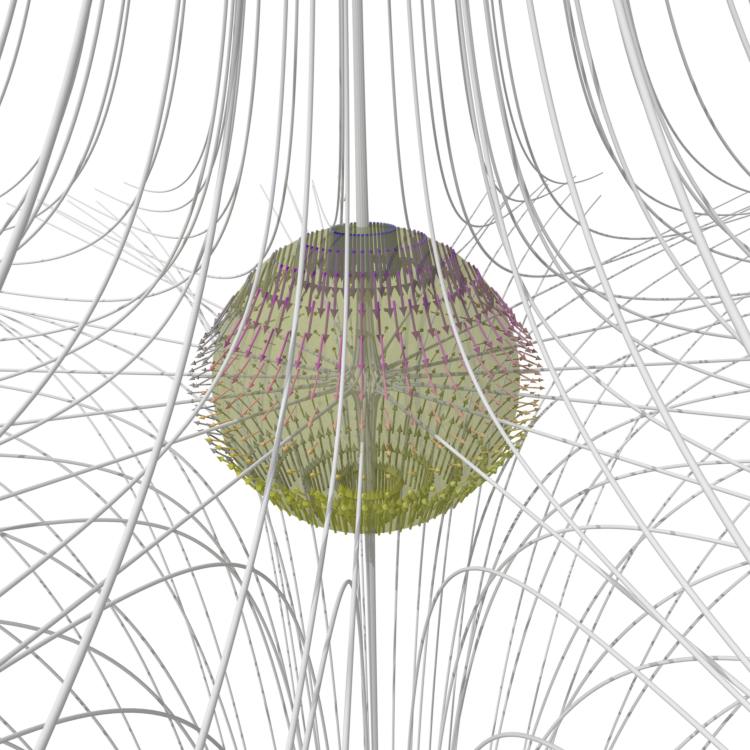
\includegraphics[width=.45\onecolwid]{fig/negindex_start.png}
        \end{figure}
        $\downarrow$
        \begin{figure}
        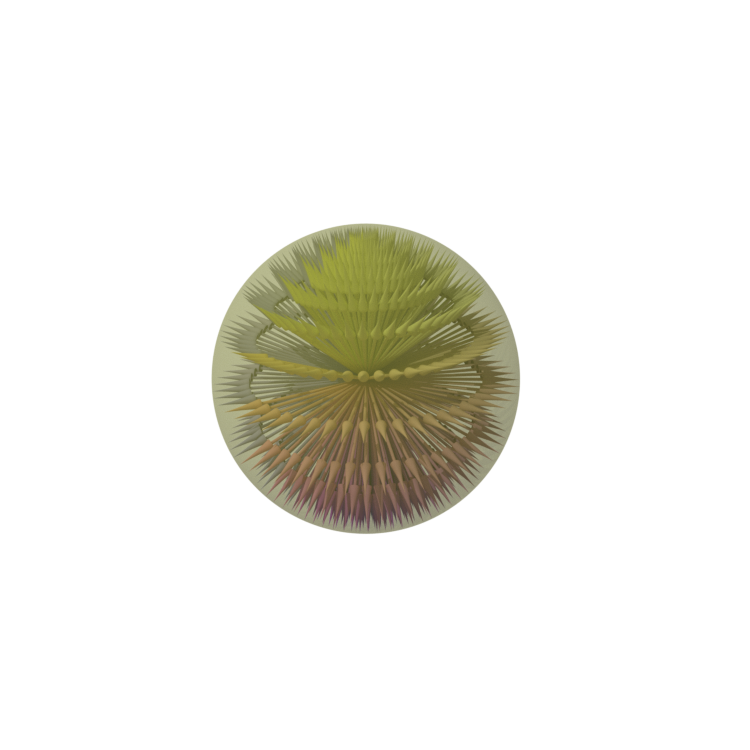
\includegraphics[width=.45\onecolwid]{fig/negindex_end.png}
        \end{figure}
        \end{centering}
    \end{column}

    \begin{column}{.45\onecolwid}
        \begin{centering}
        \textbf{Type-B}
        \begin{figure}
        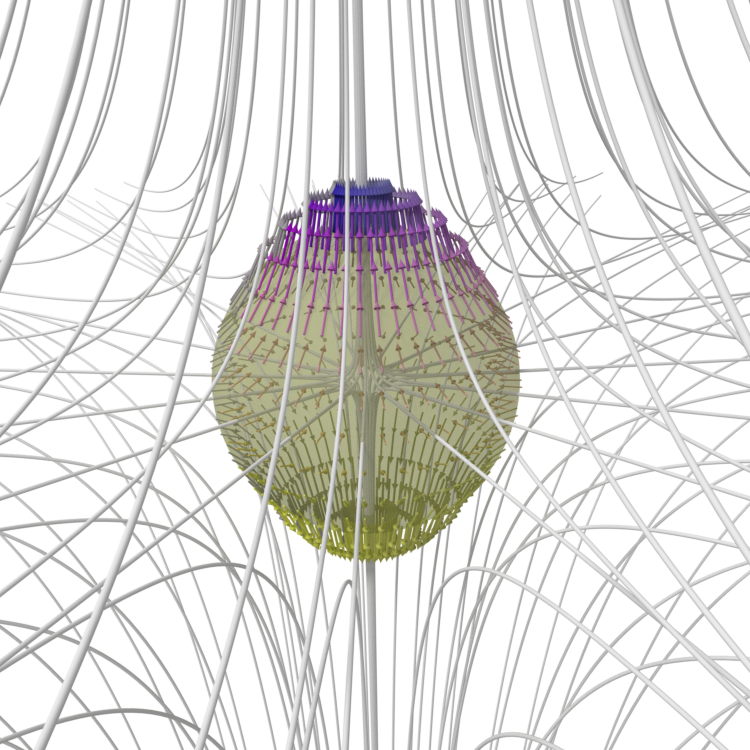
\includegraphics[width=.45\onecolwid]{fig/posindex_start.png}
        \end{figure}
        $\downarrow$
        \begin{figure}
        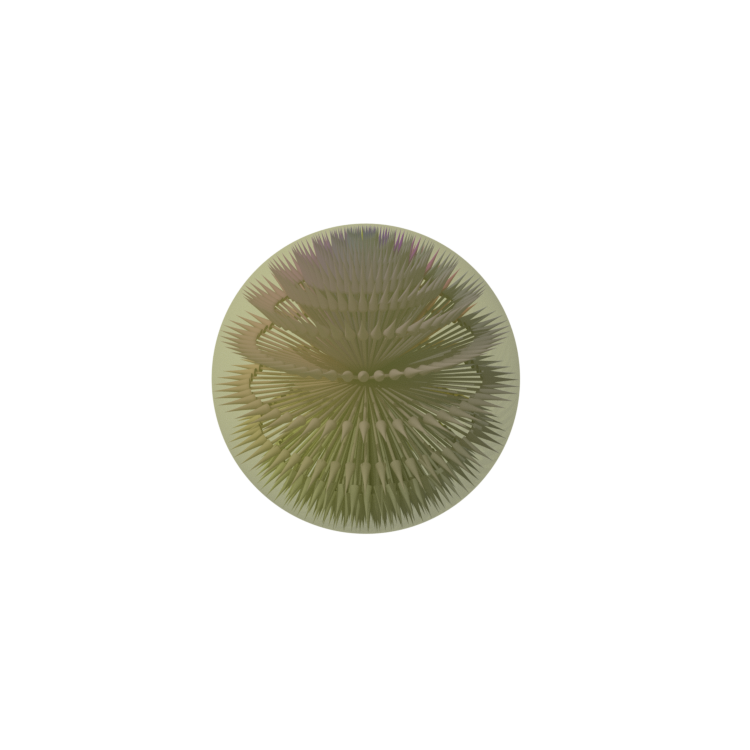
\includegraphics[width=.45\onecolwid]{fig/posindex_end.png}
        \end{figure}
    \end{centering}
    \end{column}
\end{columns}

\end{block}

%----------------------------------------------------------------------------------------

\end{column} % End of column 2.2

\end{columns} % End of the split of column 2 - any content after this will now take up 2 columns width
%----------------------------------------------------------------------------------------
%	IMPORTANT RESULT
%----------------------------------------------------------------------------------------

\begin{block}{The nulls around a dipole}
    \begin{figure}
        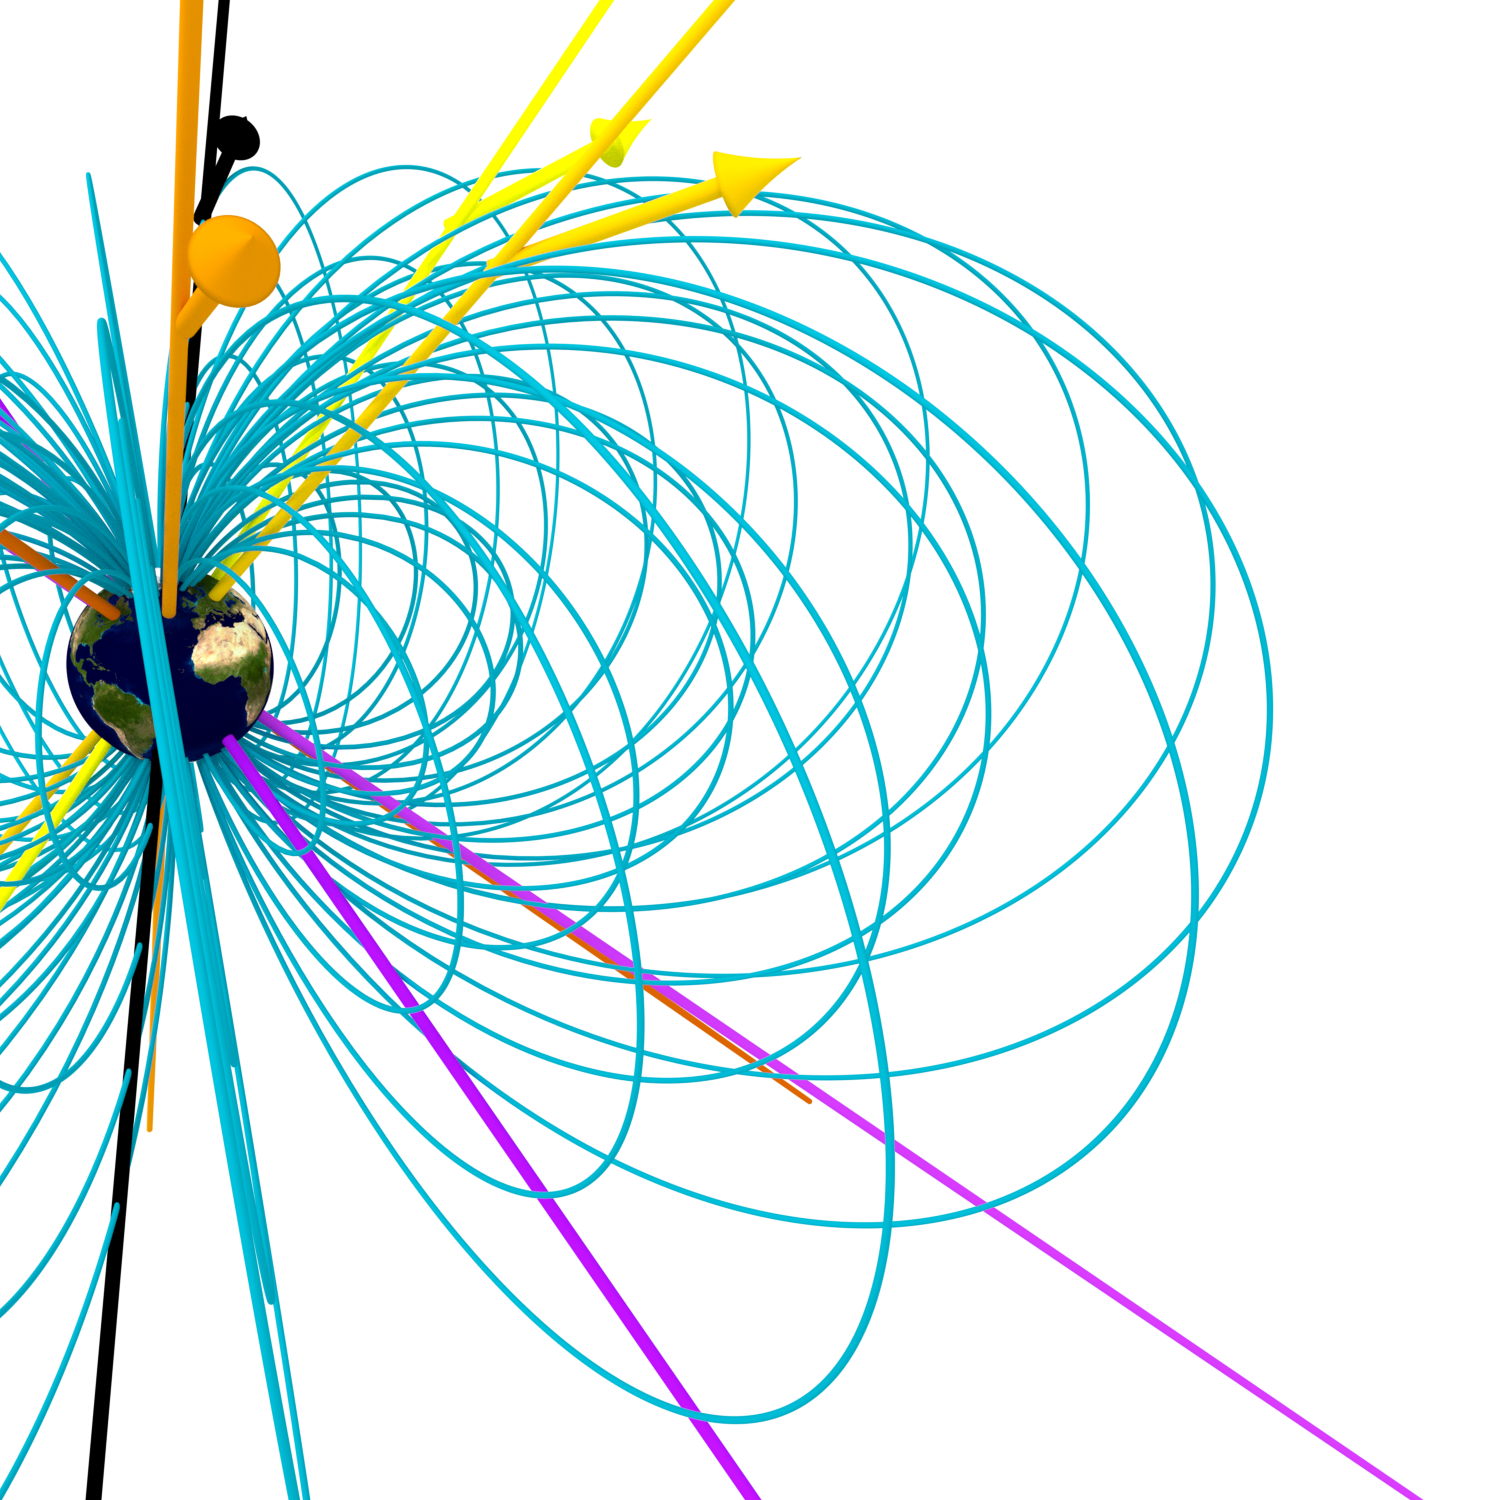
\includegraphics[width=\twocolwid]{fig/mainfig.png}
    \end{figure}

\end{block}

%----------------------------------------------------------------------------------------

\begin{columns}[t,totalwidth=\twocolwid] % Split up the two columns wide column again

\begin{column}{\onecolwid} % The first column within column 2 (column 2.1)

%----------------------------------------------------------------------------------------
%	MATHEMATICAL SECTION
%----------------------------------------------------------------------------------------

\begin{block}{Mathematical Section}

Nam quis odio enim, in molestie libero. Vivamus cursus mi at nulla elementum sollicitudin. Nam quis odio enim, in molestie libero. Vivamus cursus mi at nulla elementum sollicitudin.

\begin{equation}
E = mc^{2}
\label{eqn:Einstein}
\end{equation}

Nam quis odio enim, in molestie libero. Vivamus cursus mi at nulla elementum sollicitudin. Nam quis odio enim, in molestie libero. Vivamus cursus mi at nulla elementum sollicitudin.

\begin{equation}
\cos^3 \theta =\frac{1}{4}\cos\theta+\frac{3}{4}\cos 3\theta
\label{eq:refname}
\end{equation}

Nam quis odio enim, in molestie libero. Vivamus cursus mi at nulla elementum sollicitudin. Nam quis odio enim, in molestie libero. Vivamus cursus mi at nulla elementum sollicitudin.

\begin{equation}
\kappa =\frac{\xi}{E_{\mathrm{max}}} %\mathbb{ZNR}
\end{equation}

\end{block}

%----------------------------------------------------------------------------------------

\end{column} % End of column 2.1

\begin{column}{\onecolwid} % The second column within column 2 (column 2.2)

%----------------------------------------------------------------------------------------
%	RESULTS
%----------------------------------------------------------------------------------------


%----------------------------------------------------------------------------------------

\end{column} % End of column 1.2

\end{columns} % End of the split of column 1
\end{column} % End of the first column

\begin{column}{\sepwid}\end{column} % Empty spacer column

\begin{column}{\onecolwid} % Begin the last column


%----------------------------------------------------------------------------------------
%
%----------------------------------------------------------------------------------------

\begin{block}{The Isotropic field}
    The function $g:\mathbb{R}^3\rightarrow S^2$ used to calculate the topological index
    is a mapping from a 3-dimensional space to a two-dimensional space.
    The:


\end{block}


\begin{block}{Calculating the Iotropic field}


This statement requires citation \cite{Smith:2012qr}.

\end{block}

%----------------------------------------------------------------------------------------
\begin{block}{Source}
This poster is available under the Apache licence 2.0 and all the source material is freely
available from the Github repository at \url{https://github.com/smiet/Topological_Nulls/}.

The entire poster including all rendered graphics are created by issuing the 'make' command.
\begin{centering}
    \qrcode[height=5cm]{https://github.com/smiet/Topological_Nulls}
\end{centering}
\end{block}

\begin{block}{References}

\nocite{*} % Insert publications even if they are not cited in the poster
\small{\bibliographystyle{unsrt}
\bibliography{refs}\vspace{0.75in}}

\end{block}

\end{column} % End of the second column

\begin{column}{\sepwid}\end{column} % Empty spacer column


\end{columns} % End of all the columns in the poster

\end{frame} % End of the enclosing frame

\end{document}
